% !TeX root = ../main-presentation.tex
\begin{frame}
    \frametitle{Joint work with...}

    \begin{minipage}{0.49\textwidth}
        \centering
        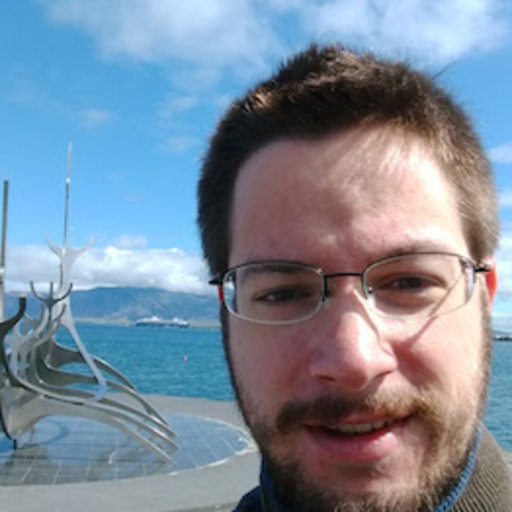
\includegraphics[width=0.5\textwidth]{imgs/sprunger}
        
        David Sprunger
    \end{minipage}
    \begin{minipage}{0.49\textwidth}
        \centering
        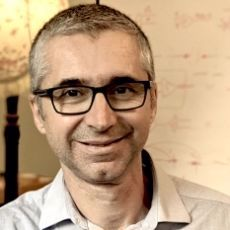
\includegraphics[width=0.5\textwidth]{imgs/ghica}
        
        Dan Ghica
    \end{minipage}

\end{frame}

\begin{frame}
    \frametitle{Introduction}
    
    Digital circuits are everywhere!

    \wait

    How do we reason with them?

\end{frame}

\begin{frame}
    \frametitle{Introduction}

    Generally by \alert{simulation}

    \wait

    Reasoning in \alert{software} is more \alert{reduction-based}:

    \[
        ((\lambda x.\lambda y.\, x + y) \, 2) \, 5 
        \wait\
        =_{\beta}
        \
        (\lambda y. 2 + y) \, 5 
        \wait\
        =_{\beta}
        \
        2 + 5 
        \wait\
        =_{\eta}
        \
        7
    \]
    
    \wait
    We want an \alert{equational theory} for digital circuits
\end{frame}